\chapter{Exercises and Code Solutions}

Two small environments. The $4\times 4$ GridWorld is tabular: the same $P$, $r$, and goal, four backups. CartPole has a continuous $s$, so a table cannot store $Q(s,a)$; DQN uses $\hat{Q}(s,a;\theta)$.

\section{Exercise 1: One GridWorld, four backups}

States $0,\ldots,15$ on a $4\times 4$ grid; $0$ is the start, $15$ is the goal (terminal). Actions are $0$ up, $1$ right, $2$ down, $3$ left. A move that would leave the grid leaves $s$ unchanged. Reward is $-1$ every step and $0$ on entering the goal.

The object to learn is a policy $\pi$, not a list of moves and not the training loop. Value-iteration sweeps and the MC, SARSA, and Q-learning episodes only \textbf{compute} $\pi$ (or $Q$, then $\pi(s)=\arg\max_a Q(s,a)$). After that, given a start state, take $\pi(s)$ at the current cell, observe $s'$, and repeat until $15$. Because $P$ is deterministic and every non-goal step costs $-1$, that walk is an \textbf{optimal trajectory} (a shortest path) from the given start to $15$. You do not re-run the backups to produce the path.

\begin{figure}[ht]
\centering
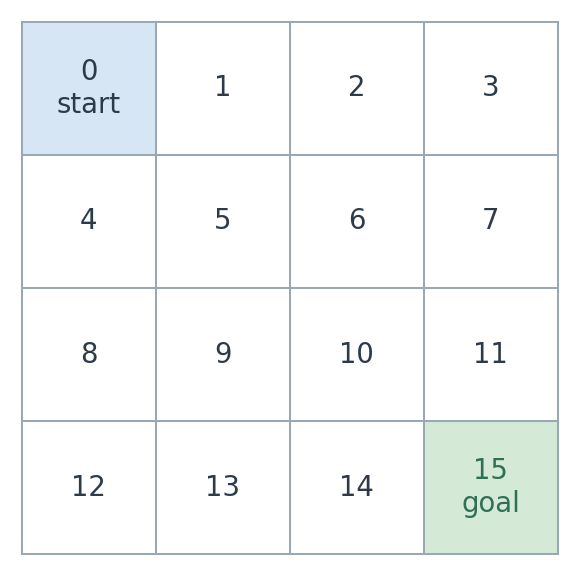
\includegraphics[width=0.42\textwidth]{gridworld_4x4.png}
\caption{GridWorld: start $0$, goal $15$ ($r=0$); every other step $r=-1$. Wall: stay in $s$. Actions: $0$ up, $1$ right, $2$ down, $3$ left.}\label{fig-14-1}
\end{figure}

The GridWorld \textbf{is} an MDP in every case. The four approaches only differ in how they compute $\pi$:

\begin{itemize}
\item \textbf{Value iteration} (dynamic programming) uses $P(s',r\mid s,a)$ and no samples.
\item \textbf{Monte Carlo control} uses samples, with target the finished $G_t$.
\item \textbf{SARSA} uses samples, with one-step target $R+\gamma Q(s',A')$ and $A'\sim\pi$ (on-policy, $Q^\pi$).
\item \textbf{Q-learning} uses samples, with one-step target $R+\gamma\max_{a'}Q(s',a')$ (off-policy, $Q^*$).
\end{itemize}
All four return a greedy $\pi(s)=\arg\max_a Q(s,a)$ (value iteration reads it from $V$). Following that $\pi$ from a start cell is the path.

\lstinputlisting{../code/ch14/gridworld_solutions.py}


VI and Q-learning typically agree on a shortest path to $15$. SARSA can differ on cells where $\varepsilon$-greedy exploration is costly. MC is noisier: its target is a full $G_t$.

\section{Exercise 2: CartPole with DQN}

The task is to \textbf{balance}: keep a pole upright on a cart that rolls on a track. The state is $s = (x, \dot{x}, \varphi, \dot{\varphi}) \in \mathbb{R}^4$: cart position and velocity, pole angle and angular velocity. The pole angle is $\varphi$, not the DQN weights $\theta$. Actions are two horizontal forces on the cart (not on the pole). If the pole is falling one way, the cart must move under it --- the same idea as balancing a stick on a palm.

Here $x$ is the cart's horizontal displacement as the cart rocks back and forth while balancing the pole. The episode ends when $\lvert x\rvert > 2.4$ or $\lvert \varphi \rvert > 12^\circ$, or after $200$ steps. Reward is $1$ every surviving step, so within one episode $G$ rises by $1$ while the pole is up. Across episodes $G$ is not monotone: $\varepsilon$-greedy still falls. $G$ cannot exceed $200$: the episode is cut there even if the pole is still up. A good $\pi$ is a plateau at $200$, not a line that keeps climbing.

The object to learn is $\pi(s)$: which force given $s$. DQN computes $\hat{Q}$, then $\pi(s) = \arg\max_a \hat{Q}(s,a;\theta)$. Acting that $\pi$ every step is how the pole stays up. You do not write a balancing formula by hand.

A table cannot store $Q(s,a)$ for every $s$. The network $\hat{Q}(s,a;\theta)$, replay $\mathcal{D}$, and frozen $\theta^-$ are the DQN update $y = r + \gamma(1-d)\max_{a'} \hat{Q}(s',a';\theta^-)$. SGD on this task is slow; Adam uses the same gradient with an adaptive step. $\varepsilon$ decays as in (6.8).

\begin{figure}[ht]
\centering
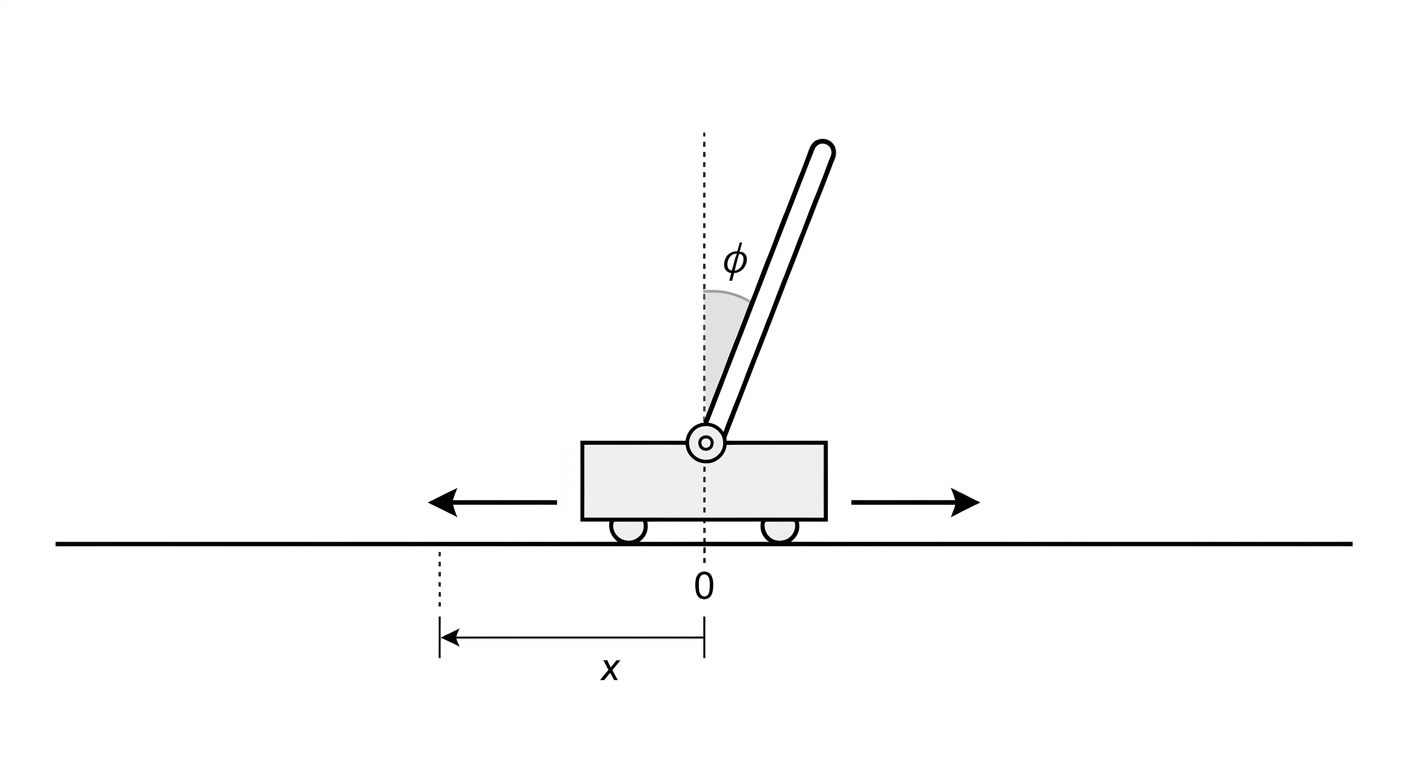
\includegraphics[width=0.72\textwidth]{cartpole.jpeg}
\caption{CartPole balancing task.}
\end{figure}

\lstinputlisting{../code/ch14/cartpole_dqn.py}


\begin{figure}[ht]
\centering
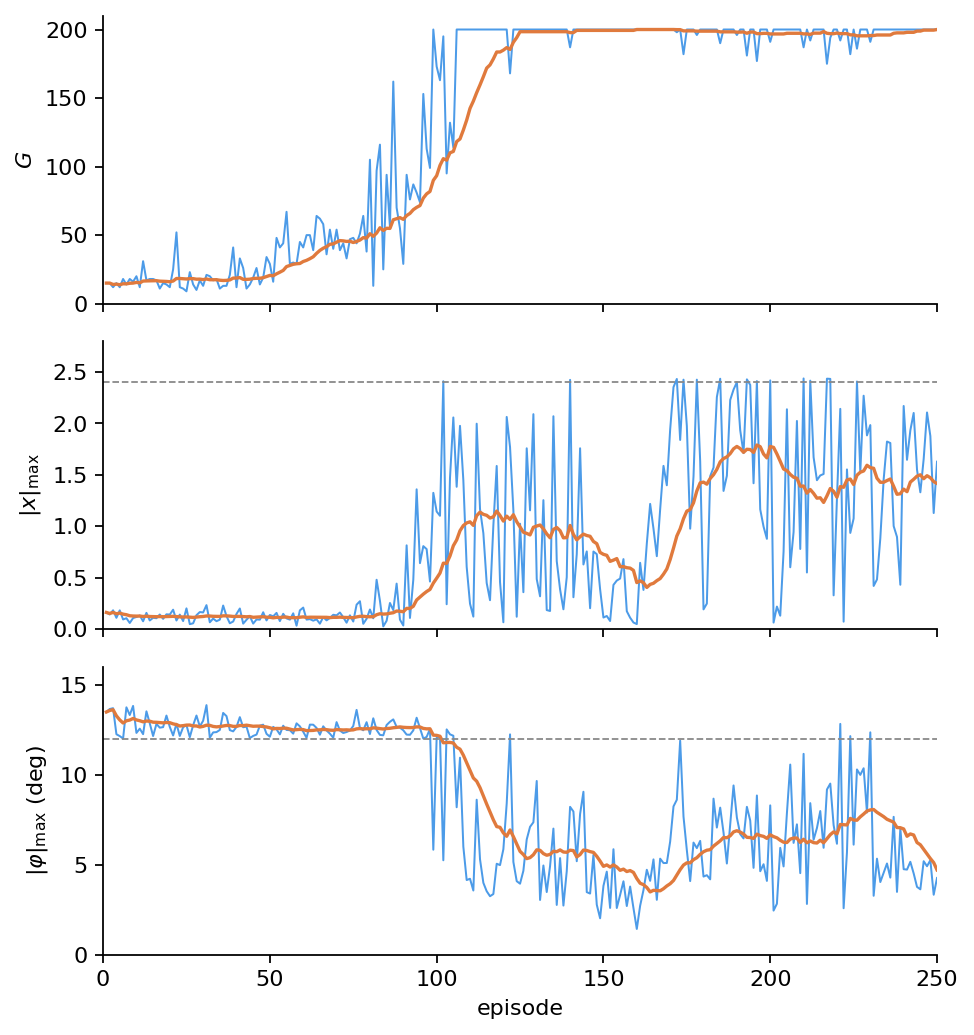
\includegraphics[width=0.72\textwidth,height=0.42\textheight,keepaspectratio]{cartpole_returns.png}
\caption{CartPole DQN, seed $0$: $G$, $|x|_{\max}$, and $|\varphi|_{\max}$ vs episode (blue) and $20$-episode mean (orange). Dashed: fail bounds $2.4$ and $12^\circ$.}\label{fig-14-2}
\end{figure}

Early $G$ near $20$ means the pole (or cart) failed after that many steps. The rise near episode $100$ is balancing starting to work. Orange $G$ flat at $200$ is the step cutoff, not unbounded gain. Late blue dips in $G$ are leftover $\varepsilon$-greedy failures.

Either bound can fail; the other need not. $|\varphi|_{\max}$ above $12^\circ$ with $|x|_{\max}$ still small is a \textbf{pole fall}: the episode stops on $\varphi$, so $x$ never reaches $2.4$. That is the early stretch. $|x|_{\max}$ on $2.4$ with $|\varphi|$ still below $12^\circ$ is a \textbf{cart} fail. The dashed lines are the fail check, not a clip: the failing coordinate can step slightly past the bound, then we stop. After learning, both stay below the dashes for $200$ steps except leftover $\varepsilon$-greedy dips.
